\documentclass[12pt]{article}

\usepackage[catalan]{babel}
\usepackage[utf8]{inputenc}
\usepackage{fancyhdr}
\usepackage{graphicx}
\usepackage[a4paper]{geometry}
\usepackage{listings}
\usepackage{multirow}
\usepackage[table,xcdraw]{xcolor}
\usepackage{hyperref}
\usepackage{float}
\usepackage{array}
\usepackage{eurosym}
\usepackage{setspace}
\usepackage{chngpage}

\pagestyle{fancy}
\fancyhf{}
\rhead{PAP}
\lhead{Designing our own cluster}
\cfoot{Pàgina \thepage}

\setlength{\parindent}{0em}
\setlength{\parskip}{1em}

\begin{document}

\makeatletter
\begin{titlepage}
\thispagestyle{empty}
\begin{center}
	\centering
	\vspace{1cm}
	{\scshape\Large Projectes de laboratori de PAP\par}
	\vspace{0.5cm}
	{\Large Curs 2019/20 (Quadrimestre de primavera)\par}
	\vspace{3cm}
	{\huge\bfseries Designing our own\par HPC-oriented cluster\par}
	\vspace{6cm}
  {\setstretch{0.25}
  {\Large \itshape Rafel-Albert Bros Esqueu\par Andrea Querol de Porras\par Joan Vinyals Ylla-Català\par Pablo Vizcaino Serrano\par}
  }
  \vspace{0.5cm}
  \vfill
	{\large Facultat d'Informàtica de Barcelona\par}
\end{center}
\clearpage
\end{titlepage}


%https://docs.google.com/spreadsheets/d/1h09R-LO8-yKG6tomeKPeug_olNzxpoOcf6uOx5kS5uo/edit?usp=sharing


%https://www.top500.org/news/cavium-releases-thunderx2-arm-processor/
%https://www.ecmwf.int/sites/default/files/elibrary/2018/18590-how-arms-entry-hpc-market-might-affect-meteorological-codes.pdf
%https://store.avantek.co.uk/avantek-64-core-cavium-thunderx2-arm-server-r281-t94.html
%https://store.avantek.co.uk/catalogsearch/result/?q=Thunderx2
%https://www.gigabyte.com/ARM-Server/Marvell-ThunderX2
%https://www.itjungle.com/2018/04/09/counting-the-cost-of-ibm-i-on-power9-entry-systems/
%https://en.wikichip.org/wiki/cavium/thunderx2/cn9980

%Power of CN9980
%https://www.servethehome.com/cavium-thunderx2-review-benchmarks-real-arm-server-option/

\section{Introducció}

En aquest projecte ens proposem dissenyar un clúster d'HPC (\textit{High Performance Computing}) obeint les restriccions establertes en la documentació. Aquestes condicions seran explicades en detall exposant, com no podria ser d'altre manera, les problemàtiques causades de cara a les decisions que caldrà prendre a l'hora d'escollir els diversos components del clúster.

\subsection{Restriccions del disseny}
En primer lloc, hi ha una restricció molt clara i sense marge per dubtes: el cost màxim per adquirir tots els components del clúster ha de ser d'un milió i mig d'euros. Això requerirà tenir ben present el preu de tots els elements i procurar no superar el límit.

L'espai també queda definit: disposem de dos armaris, cadascun d'ells de 42U i, en definitiva, 84U totals. Aquells nodes que contenen una gràfica ocuparan 2U, mentre que aquells que no en tinguin ocuparan 1U. Cal entendre que a més commutadors major serà el nombre de nodes que podem connectar a la xarxa però, paral·lelament, menor serà el nombre d'unitats que quedaran disponibles pels nodes de computació. Un cop s'hagi establert el nombre d'unitats i nodes disponibles, s'haurà de cercar la millor combinació possible entre nodes amb GPUs i nodes lliures d'elles.

Pel que fa a GPUs, el nostre disseny ve delimitat per la condició que fins a un màxim del 30\% dels flops del sistema poden provenir de nodes de computació accelerats, és a dir, de nodes amb GPUs. Tanmateix, el nombre màxim de GPUs dependrà de la placa base escollida, que al seu torn depèn del processador que haguem escollit. En definitiva: les decisions s'hauran de prendre amb peus de plom, sempre mantenint la possibilitat de fer un pas enrere i modificar qualsevol elecció prèvia.

Finalment, no existeix cap restricció específica pel que fa al consum energètic, però evidentment és important intentar maximitzar l'eficiència energètica del clúster. 

%Sou benvinguts de retocar el que us surti dels pebrots.


\section{Primeres decisions}

En aquest apartat exposarem els diversos components escollits inicialment pel nostre clúster, incloent en tot moment el procés de raonament que hem anat seguint per prendre qualsevol decisió. 
Tenint en compte que una elecció es veurà afectada per totes les prèvies, en aquesta primera fase s'han escollit diversos components candidats per a cada aspecte del clúster. Properament, els estudis per elegir els components definitius es mostraran explicats en profunditat a l'apartat d'\textit{Anàlisi}\ref{sec:analisi}.

\clearpage
\subsection{CPU}


\clearpage
\subsection{Placa base}\label{sec:motherboard}

Una vegada escollits dos processadors com a contrincants, hem començat a mirar quines plaques bases hi havia al mercat. Primerament, les hem anat buscant de manera individual i les que hem seleccionat es poden veure a la taula següent:

\begin{table}[H]
\begin{adjustwidth}{-.5in}{-.5in}  
    \begin{center}
    \centering
    \scalebox{1.0}{
\begin{tabular}{l||c|c|c|c|c|c}
    \hline
Placa mare & \begin{tabular}[c]{@{}c@{}}Nuclis \\ Màx.\end{tabular} & \begin{tabular}[c]{@{}c@{}}Storage \\ Speed\end{tabular} & \begin{tabular}[c]{@{}c@{}}DIMS \\ Màx.\end{tabular} & \begin{tabular}[c]{@{}c@{}}USB \\ 3.0\end{tabular} & PCIe 4.0 & \begin{tabular}[c]{@{}c@{}}Preu \\ (Euros)\end{tabular} \\ \hline \hline
\rowcolor[HTML]{EFEFEF}
H12DSU-iN \cite{mother1} & 64 & 6 Gbps & 32 & 5 & 1x16, 1x32, 1x40 & Coming soon \\ 
H12DST-B \cite{mother2} & 64 & 6 Gbps & 16 & 2 & 3x16, 1x24 & - \\ 
\rowcolor[HTML]{EFEFEF}
H12SSW-NT \cite{mother3} & 64 & 6 Gbps & 8 & 7 & 1x16, 1x32 & 1356.53 \cite{mother3_preu}\\
H12SSW-iN \cite{mother4} & 64 & 6 Gbps & 8 & 7 & 2x32 & - \\
\rowcolor[HTML]{EFEFEF}
H12SST-PS \cite{mother5} & 64 & 6 Gbps & 8 & 2 & 3x16 & 3959.86 \cite{mother5_preu}\\ \hline 
\end{tabular}
}
    \caption{Comparació inicial de plaques base.}
    \label{tab:_placa_base_cmp}
    \end{center}
    \end{adjustwidth}
\end{table}

Com es pot veure, les diferències principals són el número de DIMS de memòria i els PCI-Express. No obstant, una vegada fetes les comparacions inicials, ens hem adonat que per algunes d'elles era excessivament complicat trobar el preu. Per exemple, els llocs on trobàvem els preus no eren els mateixos on trobàvem les especificacions, per tant en algunes plaques no estem segurs de que els preus siguin del tot realistes.

Buscant els preus hem trobat una altra web \cite{webnodes} que ens permet crear un node seleccionant nosaltres els seus components. Hem vist que els tipus de node es diferencien inicialment entre aquells amb GPU i aquells sense GPU. Dins d'aquests dos grups trobem també els dual-socket i els single-socket.

Com que el processador \textit{AMD EPYC 7702P} té 64 nuclis i l'\textit{AMD EPYC Rome 7502P} en té 32, hem decidit plantejar-nos les opcions de nodes dual-socket amb dos processadors \textit{7502P} i nodes single-socket amb el processador \textit{7702P}. En cas d'escollir un node amb suport per GPU, ocuparem 2U en compte d'una de sola. En el cas dels nodes amb dual-socket, es poden suportar fins a 8 GPUs mentre que amb els single-socket només la meitat, 4.

\begin{figure}[H]
    \centering
    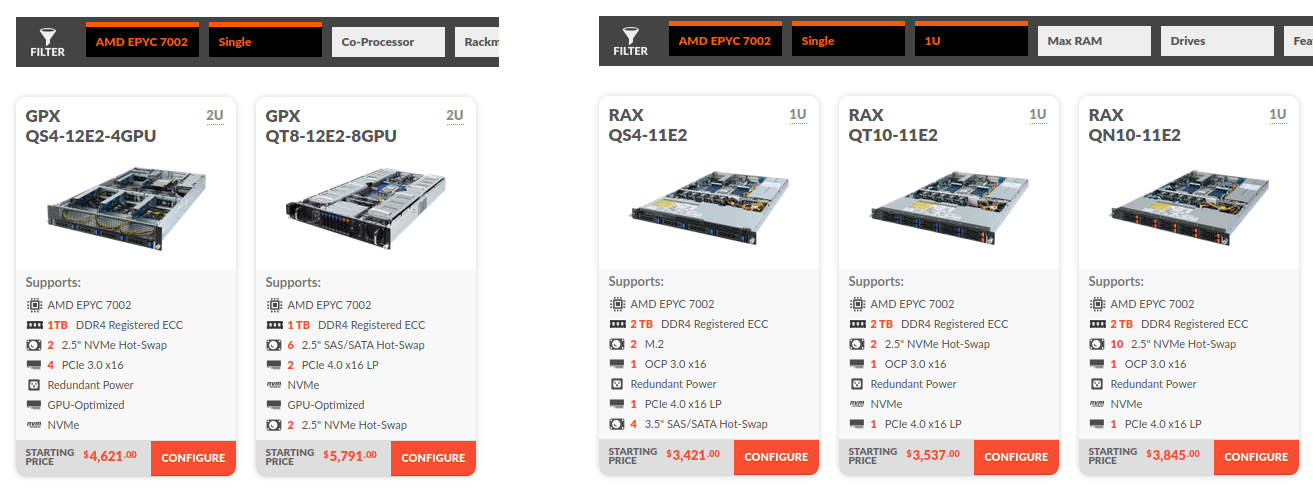
\includegraphics[width=\textwidth]{img/webnodes.png}
    \caption{Exemple de nodes que podem trobar a la web. A l'esquerra amb GPUs i a la dreta sense. Tots single-socket.}
\end{figure}

En la taula \ref{tab_web_plaques_cmp} es veuen aquestes possibles combinacions. En el cas d'utilitzar un node amb GPUs no s'ha inclòs el preu de la pròpia GPU, ja que això dependrà de quina escollim més endavant. Per la mateixa raó, tampoc s'han exposat els GFflops de les versions amb GPU. En aquests preus tampoc s'inclouen els costos de les memòries i les targetes de xarxa.

\begin{table}[h]
\begin{adjustwidth}{-.5in}{-.5in}  
    \begin{center}
    \centering
    \scalebox{1.0}{
\begin{tabular}{l||c|c|c|c|c|c}
    \hline
Configuració & Nuclis & \begin{tabular}[c]{@{}c@{}}GFlops \\ CPU\end{tabular} & GPUs & Us & \begin{tabular}[c]{@{}c@{}}Preu \\ (Euros)\end{tabular} & \begin{tabular}[c]{@{}c@{}}GFlops/ \\ Euros\end{tabular} \\ \hline \hline
 &  &  & \cellcolor[HTML]{EFEFEF}- & \cellcolor[HTML]{EFEFEF}1 & \cellcolor[HTML]{EFEFEF}9393 & \cellcolor[HTML]{EFEFEF}0.256 \\  
\multirow{-2}{*}{\begin{tabular}[l]{@{}l@{}}Dual amb AMD\\ EPYC Rome 7502P\end{tabular}} & \multirow{-2}{*}{128} & \multirow{-2}{*}{2560} & 8 & 2 & 12266 & - \\ \hline
 &  &  & \cellcolor[HTML]{EFEFEF}- & \cellcolor[HTML]{EFEFEF}1 & \cellcolor[HTML]{EFEFEF}7542 & \cellcolor[HTML]{EFEFEF}0.251 \\  
\multirow{-2}{*}{\begin{tabular}[l]{@{}l@{}}Single amb AMB\\ EPYC 7702P\end{tabular}} & \multirow{-2}{*}{128} & \multirow{-2}{*}{2048} & 4 & 2 & 9461 & - \\ \hline
\rowcolor[HTML]{EFEFEF}
\end{tabular}
}
    \caption{Comparació entre les diferents configuracions dels nodes.}
    \label{tab:web_plaques_cmp}
    \end{center}
    \end{adjustwidth}
\end{table}

Veiem que tot i que la versió amb dual-socket ens proporciona més GFlops, l'eficiència GFlops/dòllar és millor per la versió amb single-socket. Per tant, en aquest punt encara no podem decantar-nos per cap de les dues. Una vegada haguem considerat quines GPUs utilitzem, quina xarxa tenim, etc., podrem valorar si tenim suficient pressupost com per escollir la opció amb més GFlops. A més, quan les GPUs entrin en joc també s'haurà de tenir en compte que amb l'opció dual-socket en podem posar-ne el doble per cada node.



\clearpage
\subsection{Memòria RAM}

Una de les restriccions del disseny es que hem de tenir 2GB de RAM per cada core. Tenint en compte que tenim 64 cores (ja sigui amb dual-socket o amb single-socket), necessitarem 128GB de RAM. 

Hem decidit avaluar tres combinacions diferents per arribar a aquests 128GB. La primera és amb 16 DIMMs de 8GB, la segona amb 8 DIMMs de 16GB i per últim 4 DIMMs de 32GB. És més econòmic tenir menys DIMMs amb memòries de més capacitat, però limita el paral·lelisme per accedir-hi. Un altre aspecte a tenir en compte és que quants menys DIMMs utilitzem, més ens podrem expandir en un futur comprant més memòria.

També hem comparat les opcions de comprar memòria ECC (feta expressament per servidors) o NO-ECC. La diferència de preu és notable però creiem que val la pena, considerant que el pressupost no és ajustat. No hem aconseguit trobar memòries ECC de 3200Hz. En la taula següent es pot observar les memòries que hem comparat.

\begin{table}[]
\begin{tabular}{|l|l|l|l|l|l|l|l}
\hline
\cellcolor[HTML]{FFFFFF}NOM & ECC & GB & \begin{tabular}[c]{@{}l@{}}FREQ\\ (Hz)\end{tabular} & \# & Latencia & \begin{tabular}[c]{@{}l@{}}Preu(\euro)\\ (1u)\end{tabular} & \begin{tabular}[c]{@{}l@{}}Preu (\euro)\\ (Total) \end{tabular} \\ \hline
Kingston KSM29RS8\cite{mem1} & SI & 8 & 2993 & 16 & CL21 & 64.9 & 1038.4 \\ \hline
Kingston KSM29RS4\cite{mem2} & SI & 16 & 2993 & 8 & CL21 & 122.9 & 983.2 \\ \hline
Kingston KSM29RD4\cite{mem3} & SI & 32 & 2993 & 4 & CL21 & 242.9 & 971.6 \\ \hline
Kingston HyperX Impact\cite{mem4} & NO & 8 & 3200 & 16 & CL20 & 64.99 & 1039.84 \\ \hline
Kingston HyperX Impact\cite{mem5} & NO & 16 & 3200 & 8 & CL20 & 107.99 & 863.92 \\ \hline
Kingston HyperX Fury Black\cite{mem6} & NO & 32 & 3200 & 4 & CL16 & 169.0 & 676 \\ \hline
\end{tabular}
\caption{Comparació de les diferents memòries estudiades}
\end{table}

Hem decidit decantar-nos per la versió amb 8 DIMMs de 16GB. Creiem que té un bon balanceig entre paral·lelisme, possible extensió i preu. Com estem dins el pressupost, hem escollit la versió ECC.

\clearpage
\subsection{Xarxa d'interconnexió}

Entenent que tenim un nombre relativament reduït d'unitats i que volem dedicar tantes unitats com 
sigui possible a nodes de còmput, volem reduir el nombre d'unitats que dediquem als commutadors. Per aconseguir aquesta fita, necessitem que cada commutador tingui el màxim
nombre de ports per unitat.
Com efecte col·lateral d'aquesta estratègia ens veiem amb un sistema que pràcticament es veu forçat a utilitzar una topologia de xarxa de tipus malla.

Pel que fa a distribuïdors, ens vam centrar en \textit{Mallanox Technologies}. A la pàgina web
\cite{mellanox-web} de la companyia, vam trobar commutadors \textit{InfiniBand} de diferents preus
i velocitats (com més ports major és la velocitat). A la taula \ref{tab:intercon} hem recollit els 
diferents models candidats a ser utilitzats en el nostre sistema.

\begin{table}[H]
\begin{adjustwidth}{-.5in}{-.5in}  
    \begin{center}
        \centering
        \scalebox{1.0}{
        \begin{centering}
            \begin{tabular}{l||c|c|c}
                \hline
                \cellcolor[HTML]{FFFFFF}Model         & Ports & Speed (Gb/s) & Preu (\$) \\ \hline \hline \rowcolor[HTML]{EFEFEF}
                MSX6012F-2BFS \cite{mellanox_msx6012f-2bfs} & 12      & 56           &  9309.00  \\ 
                MSX6018F-1SFS \cite{mellanox_msx6018f-1sfs} & 18      & 56           & 14791.00  \\ \rowcolor[HTML]{EFEFEF} 
                MSB7800-ES2F \cite{mellanox_msb7800-es2f}  & 36      & 100          & 25633.00  \\ 
                MQM8700-HS2F \cite{mellanox_mqm8700-hs2f}  & 40      & 200          & 29629.00  \\ \hline
            \end{tabular}
        \end{centering}
        }
    \caption{Comparació entre les diferents configuracions dels nodes.}
    \label{tab:intercon}
    \end{center}
\end{adjustwidth}
\end{table}

La quantitat de commutadors que utilitzem en el nostre sistema és un factor clau que marca,
tan el preu, com el rendiment, d'aquest. D'altre banda, però, afecta diferent als dos paràmetres,
anteriors en funció dels altres components. Per tan no podem determinar encara quina serà la
millor configuració. No obstant, si que podem reduir el rang de configuracions, per tal que
l'anàlisi sigui més amè.

Ja que utilitzem una topologia de tipus malla completa, el nombre de connexions $C$ a nodes de còmput
que podrà tenir la xarxa ve marcat per el nombre de ports $P$ del que disposa cada commutador, així
com el nombre de commutadors $N$ que tingui el sistema. Deduïm que el nombre de connexions
que podrà haver al sistema ve determinat per $C = N \times ( P - N + 1 ) = -N^2 + N(P+1)$.
A la figura \ref{fig:connections} podem veure quin és el comportament d'aquesta funció quan incrementem
el nombre de commutadors, aquesta figura consta del comportament dels commutadors, així com del nombre 
d'unitats que queden disponibles. Pel nostre sistema estudiarem aquelles configuracions que s'acostin 
més a la línia de punts. Cal entendre que si són més avall de la línia de punts vol dir que estem perden connexions
i que possiblement ens quedi espai lliure a l'armari. D'altra banda, si som més amunt de la línia 
significa que ja tenim les connexions necessàries per omplir els dos armaris; incrementar el nombre de connexions
només ens portaria a desaprofitar-les (assumim que mínim una U per node).

Llavors, a partir d'aquest argument podem desglossar les diferents configuracions que val la pena explorar:
\begin{itemize}
  \item El cas del model \textit{MSX6012F-2BFS} no l'analitzarem, ja que no hi ha cap configuració òptima per la topologia utilitzada.
  \item Pel cas del model \textit{MSX6018F-1SFS}, tenint en compte que tenim divuit ports, analitzarem les configuracions amb sis i set commutadors.
  \item Pel cas del model \textit{MSB7800-ES2F}, amb trenta-sis ports, centrarem l'anàlisi en les configuracions de dos i tres commutadors.
  \item Pel cas del model \textit{MQM8700-HS2F}, amb quaranta ports, ens centrarem també en dos i tres commutadors.
\end{itemize}

\begin{figure}[h!]
    \centering
    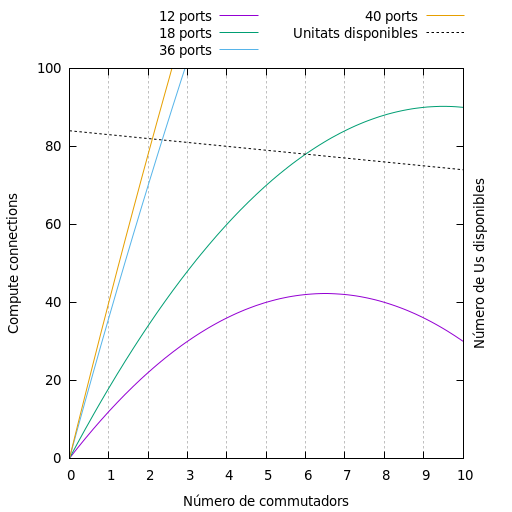
\includegraphics[width=0.8\linewidth]{img/connections.png}
    \caption{Caption}
    \label{fig:connections}
\end{figure}



\clearpage
\subsection{GPU}

Finalment, queda plantejar-nos l'últim element pel nostre clúster: les unitats de processament gràfic o GPUs. Un cop més, el procediment ha estat buscar diverses GPUs candidates i comparar les seves característiques bolcant-les en una taula, tal com es pot veure a continuació:

\begin{table}[H]
\begin{adjustwidth}{-1.0in}{-1.0in}  
    \begin{center}
    \centering
    \scalebox{0.8}{
\begin{tabular}{cc||c|c|c|c|c|c|c}
    \hline
\multicolumn{2}{c||}{Model}                                                                                                 & \begin{tabular}[c]{@{}c@{}}\cellcolor[HTML]{FFFFFF}NVIDIA \\ Tesla \\ V100\end{tabular} & \begin{tabular}[c]{@{}c@{}}NVIDIA \\ RTX \\ 2080 TI\end{tabular} & \begin{tabular}[c]{@{}c@{}}NVIDIA \\ Quadro RTX \\ 8000\end{tabular} & \begin{tabular}[c]{@{}c@{}}NVIDIA \\ Tesla \\ T4\end{tabular} & \begin{tabular}[c]{@{}c@{}}AMD Radeon \\ Pro WX \\ 8200\end{tabular} & \begin{tabular}[c]{@{}c@{}}AMD Radeon \\ Instinct \\ MI50\end{tabular} & \begin{tabular}[c]{@{}c@{}}AMD Radeon \\ Instinct \\ MI25\end{tabular} \\ \hline \hline
& \cellcolor[HTML]{EFEFEF}Preu (\$)                                                     & \cellcolor[HTML]{EFEFEF}7,399.00                                & \cellcolor[HTML]{EFEFEF}1,159.99                                 & \cellcolor[HTML]{EFEFEF}4,902.00                                     & \cellcolor[HTML]{EFEFEF}2199                                  & \cellcolor[HTML]{EFEFEF}969.99                                       & \cellcolor[HTML]{EFEFEF}4,438.00                                       & \cellcolor[HTML]{EFEFEF}9156.65                                        \\
                                 \hline & {Power (W)}                                                                              & 300                                                             & 250                                                              & 260                                                                  & 70                                                            & 230                                                                  & 300                                                                    & 300                                                                    \\
                                 \hline
                                  & \cellcolor[HTML]{EFEFEF}Freq (MHz)                                                     & \cellcolor[HTML]{EFEFEF}1246                                    & \cellcolor[HTML]{EFEFEF}1350                                     & \cellcolor[HTML]{EFEFEF}1395                                         & \cellcolor[HTML]{EFEFEF}585                                   & \cellcolor[HTML]{EFEFEF}1200                                         & \cellcolor[HTML]{EFEFEF}1200                                           & \cellcolor[HTML]{EFEFEF}1400                                           \\ \hline
                                  & Type                                                                                   & hbm2                                                            & gddr6                                                            & gddr6                                                                & gddr6                                                         & hbm2                                                                 & hbm2                                                                   & hbm2                                                                   \\
                                  & \cellcolor[HTML]{EFEFEF}GB                                                             & \cellcolor[HTML]{EFEFEF}16 o 32                                 & \cellcolor[HTML]{EFEFEF}11                                       & \cellcolor[HTML]{EFEFEF}48                                           & \cellcolor[HTML]{EFEFEF}16                                    & \cellcolor[HTML]{EFEFEF}8                                            & \cellcolor[HTML]{EFEFEF}32                                             & \cellcolor[HTML]{EFEFEF}16                                             \\
\multirow{-3}{*}{Memòria}             & \begin{tabular}[c]{@{}c@{}}Bandwidth\\ (GB/s)\end{tabular}                             & 900                                                             & 616                                                              & 672                                                                  & 320                                                           & 512                                                                  & 1024                                                                   & 484                                                                    \\ \hline
                                  & \cellcolor[HTML]{EFEFEF}Interface                                                      & \cellcolor[HTML]{EFEFEF}PCIe 3.0                                & \cellcolor[HTML]{EFEFEF}PCIe 3.0                                 & \cellcolor[HTML]{EFEFEF}PCIe 3.0                                     & \cellcolor[HTML]{EFEFEF}PCIe 3.0                              & \cellcolor[HTML]{EFEFEF}PCIe 3.0                                     & \cellcolor[HTML]{EFEFEF}PCIe 3.0 \& 4.0                           & \cellcolor[HTML]{EFEFEF}PCIe3.0                                        \\
                                  & Lanes                                                                                  & 16                                                              & 16                                                               & 16                                                                   & 16                                                            & 16                                                                   & 16                                                                     & 16                                                                     \\
\multirow{-3}{*}{Interconnexió} & \cellcolor[HTML]{EFEFEF}\begin{tabular}[c]{@{}c@{}}Bandwidth \\ (GB/s)\end{tabular} & \cellcolor[HTML]{EFEFEF}32                                      & \cellcolor[HTML]{EFEFEF}32                                       & \cellcolor[HTML]{EFEFEF}32                                           & \cellcolor[HTML]{EFEFEF}32                                    & \cellcolor[HTML]{EFEFEF}32                                           & \cellcolor[HTML]{EFEFEF}32                                             & \cellcolor[HTML]{EFEFEF}32                                             \\ \hline
                                  &  GFlops                                                                                 & 7,235.58                                                        & 420.20                                                           & 509.80                                                               & 254.40                                                        & 672.00                                                               & 6,865.92                                                               & 768.00                                                                 \\
                                  & \cellcolor[HTML]{EFEFEF}GFlops/W                                                       & \cellcolor[HTML]{EFEFEF}24.12                                   & \cellcolor[HTML]{EFEFEF}1.68                                     & \cellcolor[HTML]{EFEFEF}1.96                                         & \cellcolor[HTML]{EFEFEF}3.63                                  & \cellcolor[HTML]{EFEFEF}2.92                                         & \cellcolor[HTML]{EFEFEF}22.89                                          & \cellcolor[HTML]{EFEFEF}2.56                                           \\
\multirow{-3}{*}{FP64}            & GFlops/\$                                                                              & 0.98                                                            & 0.36                                                             & 0.10                                                                 & 0.12                                                          & 0.69                                                                 & 1.55                                                                   & 0.08                                                                   \\ \hline
                                  & \cellcolor[HTML]{EFEFEF}GFlops                                                         & \cellcolor[HTML]{EFEFEF}14,469.12                               & \cellcolor[HTML]{EFEFEF}13,772.80                                & \cellcolor[HTML]{EFEFEF}16,701.44                                    & \cellcolor[HTML]{EFEFEF}8,336.38                              & \cellcolor[HTML]{EFEFEF}11,008.00                                    & \cellcolor[HTML]{EFEFEF}13,731.84                                      & \cellcolor[HTML]{EFEFEF}12,584.96                                      \\
                                  & GFlops/W                                                                               & 48.23                                                           & 55.09                                                            & 64.24                                                                & 119.09                                                        & 47.86                                                                & 45.77                                                                  & 41.95                                                                  \\
\multirow{-3}{*}{FP32}            & \cellcolor[HTML]{EFEFEF}GFlops/\$                                                      & \cellcolor[HTML]{EFEFEF}1.96                                    & \cellcolor[HTML]{EFEFEF}11.87                                    & \cellcolor[HTML]{EFEFEF}3.41                                         & \cellcolor[HTML]{EFEFEF}3.79                                  & \cellcolor[HTML]{EFEFEF}11.35                                        & \cellcolor[HTML]{EFEFEF}3.09                                           & \cellcolor[HTML]{EFEFEF}1.37                                           \\ \hline
                                  & GFlops                                                                                 & 28938.24                                                        & 27545.60                                                         & 33402.88                                                             & 66693.12                                                      & 2201.60                                                              & 27463.68                                                               & 25169.92                                                               \\
                                  & \cellcolor[HTML]{EFEFEF}GFlops/W                                                       & \cellcolor[HTML]{EFEFEF}96.46                                   & \cellcolor[HTML]{EFEFEF}110.18                                   & \cellcolor[HTML]{EFEFEF}128.47                                       & \cellcolor[HTML]{EFEFEF}952.76                                & \cellcolor[HTML]{EFEFEF}9.57                                         & \cellcolor[HTML]{EFEFEF}91.55                                          & \cellcolor[HTML]{EFEFEF}83.90                                          \\
\multirow{-3}{*}{FP16}            & GFlops/\$                                                                              & 3.91                                                            & 23.75                                                            & 6.81                                                                 & 30.33                                                         & 2.27                                                                 & 6.19                                                                   & 2.75 \\ \hline
\end{tabular}
    }
\end{center}
\end{adjustwidth}
    \caption{Característiques de les diverses targetes gràfiques estudiades.}
    \label{tab:gpu_specs}
\end{table}


\section{Anàlisi de possibles configuracions}

Arribats a aquest punt, hem deixat moltes eleccions de components al aire ja que depenen unes de les altres. Per a poder valorar-les correctament, hem decidit provar-les totes amb l'ajut de fulls de càlcul que es poden trobar a l'annex.

Les combinacions de components que tenim són les següents:
\begin{itemize}
    \item {Nodes single-socket (cpu 7702) o dual-socket (cpu 7502)}
    \item {Nodes amb o sense gràfiques}
    \item {7 gràfiques diferents}
    \item {3 commutadors diferents amb 4 possibles combinacions de xarxa}
\end{itemize}



Per a cada una de les xarxes (nombre i tipus de commutador) s'ha estudiat quina és la combinació de nodes sense gràfica (1U) i amb gràfica (2U) que ens maximitza els TFLOPS, complint la restricció del percentatge dels TFLOPS que poden representar de les gràfiques. S'ha considerat que els nodes que tenen gràfica ocupen tots els possibles slots per aquestes, i així s'optimitza millor l'espai. En la següent taula es poden veure els resultats resumits (és a dir, per cada combinació de nodes dins la xarxa s'ha mostrat només la que otorga més TFLOPS), però si es vol veure totes les possibles combinacions es pot anar a l'annex.

\begin{table}[H]
\begin{adjustwidth}{-1.0in}{-1.0in}
\begin{center}
\begin{tabular}{ll|c|c|c|c}
\cline{3-6}
{\color[HTML]{000000} } & {\color[HTML]{000000} } & \multicolumn{4}{c|}{{\color[HTML]{000000} {[}Commutadors{]} x {[}Ports{]}}} \\ \cline{3-6} 
{\color[HTML]{000000} } & {\color[HTML]{000000} } & {\color[HTML]{000000} 6x18} & {\color[HTML]{000000} 7x18} & {\color[HTML]{000000} 3x36} & {\color[HTML]{000000} 3x40} \\ \hline
\multicolumn{1}{l|}{{\color[HTML]{000000} }} & \multicolumn{1}{l||} {\cellcolor[HTML]{EFEFEF} Nodes 1U} & {\cellcolor[HTML]{EFEFEF} 72} & {\cellcolor[HTML]{EFEFEF} 71} & {\cellcolor[HTML]{EFEFEF} 75} & {\cellcolor[HTML]{EFEFEF} 75} \\ 
\multicolumn{1}{l|}{{\color[HTML]{000000} }} & \multicolumn{1}{l||}{\color[HTML]{000000} Nodes 2U} & {\color[HTML]{000000} 3} & {\color[HTML]{000000} 3} & {\color[HTML]{000000} 3} & {\color[HTML]{000000} 3} \\ 
\multicolumn{1}{l|}{{\color[HTML]{000000}} } & \multicolumn{1}{l||} {\cellcolor[HTML]{EFEFEF} Gràfiques} & {\cellcolor[HTML]{EFEFEF}} \begin{tabular}[c]{@{}c@{}}NVIDIA \\ tesla V100\end{tabular} & {\cellcolor[HTML]{EFEFEF} \begin{tabular}[c]{@{}c@{}}AMD Radeon\\ Instinct MI50\end{tabular}} & {\cellcolor[HTML]{EFEFEF} \begin{tabular}[c]{@{}c@{}}NVIDIA\\ tesla V100\end{tabular}} & {\cellcolor[HTML]{EFEFEF} \begin{tabular}[c]{@{}c@{}}NVIDIA\\ tesla V100\end{tabular}} \\
\multicolumn{1}{l|}{{\color[HTML]{000000} }} & \multicolumn{1}{c||}{\color[HTML]{000000} TFlops} & {\color[HTML]{000000} 213.594} & {\color[HTML]{000000} 208.345} & {\color[HTML]{000000} 219.594} & {\color[HTML]{000000} 219.594} \\
\multicolumn{1}{c|}{{\color[HTML]{000000} }} & \multicolumn{1}{c||} {\cellcolor[HTML]{EFEFEF} Preu (\euro)} & {\cellcolor[HTML]{EFEFEF} 847263} & {\cellcolor[HTML]{EFEFEF} 826255.8} & {\cellcolor[HTML]{EFEFEF} 892893.6} & {\cellcolor[HTML]{EFEFEF} 973131.6} \\
\multicolumn{1}{l|}{\multirow{-6}{*}{{\color[HTML]{000000} \begin{tabular}[l]{@{}l@{}}Single-Socket\\ AMD 7702\end{tabular}}}} & \multicolumn{1}{l||}{\color[HTML]{000000} Gflops/\euro} & {\color[HTML]{000000} 0.258} & {\color[HTML]{000000} 0.258} & {\color[HTML]{000000} 0.252} & {\color[HTML]{000000} 0.231} \\ \hline
\multicolumn{1}{l|}{{\cellcolor[HTML]{FFFFFF} }} & \multicolumn{1}{l||} {\cellcolor[HTML]{EFEFEF} Nodes 1U} & {\cellcolor[HTML]{EFEFEF} 74} & {\cellcolor[HTML]{EFEFEF} 73} & {\cellcolor[HTML]{EFEFEF} 77} & {\cellcolor[HTML]{EFEFEF} 77} \\ 
\multicolumn{1}{l|}{{\color[HTML]{000000} }} & \multicolumn{1}{l||}{\color[HTML]{000000} Nodes 2U} & {\color[HTML]{000000} 2} & {\color[HTML]{000000} 2} & {\color[HTML]{000000} 2} & {\color[HTML]{000000} 2} \\ 
\multicolumn{1}{l|}{{\color[HTML]{000000} }} & \multicolumn{1}{c||} {\cellcolor[HTML]{EFEFEF} Gràfiques} & {\cellcolor[HTML]{EFEFEF} \begin{tabular}[c]{@{}l@{}}AMD Radeon\\ Instinct MI50\end{tabular}} & {\cellcolor[HTML]{EFEFEF} \begin{tabular}[c]{@{}l@{}}NVIDIA\\ tesla V100\end{tabular}} & {\cellcolor[HTML]{EFEFEF} \begin{tabular}[c]{@{}l@{}}AMD Radeon\\ Instinct MI50\end{tabular}} & {\cellcolor[HTML]{EFEFEF} \begin{tabular}[c]{@{}l@{}}AMD Radeon\\ Instinct MI50\end{tabular}} \\
\multicolumn{1}{l|}{{\color[HTML]{000000} }} & \multicolumn{1}{c||} {\color[HTML]{000000} TFlops} & {\color[HTML]{000000} 270.46} & {\color[HTML]{000000} 258.16} & {\color[HTML]{000000} 277.96} & {\color[HTML]{000000} 277.96} \\
\multicolumn{1}{l|}{{\color[HTML]{000000} }} & \multicolumn{1}{c||} {\cellcolor[HTML]{EFEFEF} Preu (\euro)} & {\cellcolor[HTML]{EFEFEF} 983231.2} & {\cellcolor[HTML]{EFEFEF} 1007763} & {\cellcolor[HTML]{EFEFEF} 1034778.8} & {\cellcolor[HTML]{EFEFEF} 1034778.8} \\ 
\multicolumn{1}{l|}{\multirow{-6}{*}{{\color[HTML]{000000} \begin{tabular}[c]{@{}l@{}}Dual-Socket\\ AMD-7502\end{tabular}}}} & \multicolumn{1}{c||} {\color[HTML]{000000} Gflops/\euro} & {\color[HTML]{000000} 0.282} & {\color[HTML]{000000} 0.262} & {\color[HTML]{000000} 0.275} & {\color[HTML]{000000} 0.255} \\ \hline
\end{tabular}
\caption{Mostra de les diverses combinacions valorades.}
\end{center}
\end{adjustwidth}
\end{table}

En primer lloc, analitzem la taula en el eix horitzontal. S'observa que els TFLOPS que ens dóna utilitzar 3 commutadors de 36 ports i 3 de 40 són els mateixos. Això es perquè amb la primera opció ja tenim suficients ports com per emplenar els racks amb tots els nodes que hi caben. La millora d'utilizar els commutadors de 40 ports és que tenen una velocitat més bona, 200Gbits en comptes de 100. El preu puja, però ens ho podem permetre.

Per altra banda, observem que amb 6 commutadors de 18 ports aconseguir una eficiència Gflops/\euro més bona, tot i que no arribem a tants TFLOPS com amb altres opcions.

Analitzant la taula en l'eix vertical, veiem que per qualsevol configuració la versió amb Dual-Socket ens dóna més TFLOPS amb una eficiència econòmica millor. Això pot ser degut en part a que els nodes amb gràfiques poden tenir-ne fins a 8 per node en comptes de 4 com en el cas del Single-Socket. Per tant, podem tenir més gràfiques utilitzant menys Us, deixant-ne més disponibles per a nodes sense gràfiques (1U).



\section{Clúster final}
Veient les opcions presentades en la secció anterior,  hem decidit escollir la versió que ens dóna més TFlops. Aquesta és la que té nodes dual-socket amb el processador \textit{7502}. Hem escollit comprar els commutadors de quaranta ports ja que ens ofereixen el doble de velocitat que els de trenta-sis (200 Gbits i 100 Gbits respectivament).

Podem veure que el percentatge de TFlops de les gràfiques respecte el total és 0.289. Aquest número s'aconseguia amb dotze GPUs, posant sis en dos nodes. Com els nodes tenen vuit slots per gràfiques, podríem afegir quatre gràfiques amb menys TFlops i intentar apropar-nos més al 30\% de TFlops de GPU que ens imposa la restricció.

Per fer-ho, afegim quatre gràfiques \textit{AMD Radeon Pro WX8200}, afegint 2.625 TFlops al nostre clúster. El preu s'incrementa en 3879.96\$ i el ràtio de TFlops GPU/Total acaba sent 0.296.

Més concretament, aquesta és la configuració que hem escollit:
\begin{table}[H]
\begin{adjustwidth}{-1.0in}{-1.0in}
\begin{center}
\begin{tabular}{l|l}
\hline
{\cellcolor[HTML]{EFEFEF}CPU}         & {\cellcolor[HTML]{EFEFEF}Dual-Socket AMD EPYC Rome 7502P} \\ 
Cores/Node                                       & 128                                             \\ 
{\cellcolor[HTML]{EFEFEF}GPU\_1}                       & {\cellcolor[HTML]{EFEFEF}AMD Radeon Instinct MI50} \\ 
\#GPU\_1                                           & 12 (2 nodes amb 6 GPUs)                         \\
{\cellcolor[HTML]{EFEFEF}GPU\_2}                       & {\cellcolor[HTML]{EFEFEF}AMD RadeonPro WX8200} \\ 
\#GPU\_2                                           & 4 (2 nodes amb 2 GPUs)                         \\
{\cellcolor[HTML]{EFEFEF}Memòria}     & {\cellcolor[HTML]{EFEFEF}Kingston KSM29RS4 DDR4 2933Hz}   \\
{\color[HTML]{000000}Memòries/node}             & {\color[HTML]{000000}8 DIMMS de 16GB}          \\ 
{\cellcolor[HTML]{EFEFEF}Commutadors} & {\cellcolor[HTML]{EFEFEF}Mellanox MQM8700-HS2F, 200Gbits} \\ 
{\color[HTML]{000000}\#Commutadors}             & {\color[HTML]{000000}3}                        \\ 
{\cellcolor[HTML]{EFEFEF}\#Nodes sense GPU (1U)}    & {\cellcolor[HTML]{EFEFEF}77}                       \\
{\color[HTML]{000000}\#Nodes amb GPU (2U)}      & {\color[HTML]{000000}2}                        \\
{\cellcolor[HTML]{EFEFEF}Us de nodes}               & {\cellcolor[HTML]{EFEFEF}81}                       \\
{\color[HTML]{000000}Us de nodes + commutadors} & {\color[HTML]{000000}84}                       \\
{\cellcolor[HTML]{EFEFEF}TFlops CPU}                & {\cellcolor[HTML]{EFEFEF}197.5}                    \\
{\color[HTML]{000000}TFlops GPU}                & {\color[HTML]{000000}83.085}                    \\ 
{\cellcolor[HTML]{EFEFEF}TFlops Totals}             & {\cellcolor[HTML]{EFEFEF}280.585}                   \\ 
{\color[HTML]{000000}TFlops GPU/Totals}         & {\color[HTML]{000000} 0.296}                    \\ 
{\cellcolor[HTML]{EFEFEF}Cost (Dòllars)}                 & {\cellcolor[HTML]{EFEFEF}1127027.41}              \\
{\color[HTML]{000000}GFlops/Dòllar}               & {\color[HTML]{000000}0.255}                    \\ \hline
\end{tabular}
\caption{Configuració final del clúster}
\end{center}
\end{adjustwidth}
\end{table}




\subsection{Roofline}






\bibliographystyle{unsrt}
\bibliography{cluster}


\end{document}
